\documentclass{article}
\usepackage{amsmath}
\usepackage{tikz}
\tikzstyle{every picture}+=[remember picture]
\usetikzlibrary{matrix}

\usepackage{gauss2}
% patch gauss macros for doing their work in `align'
% and other amsmath environments; see
% http://tex.stackexchange.com/questions/146532/
\usepackage{etoolbox}
\makeatletter
\patchcmd\g@matrix
 {\vbox\bgroup}
 {\vbox\bgroup\normalbaselines}% restore the standard baselineskip
 {}{}

\edef\g@post{\relax$} % $ 
\newdimen\colwidth
\def\arrowheight{\g@dim{cx1}{\colwidth}}
\newdimen\rowheight
\def\arrowwidth{\g@dim{cy1}{\rowheight}}
\def\gvline{\g@vline}
\newdimen\sumen
\let\gsetdim=\g@defdim
\let\gmaxcol=\g@maxcol
\let\gmaxrow=\g@maxrow
\let\gdouble=\g@double
\let\gdefdouble=\g@defdouble
\let\gadvance=\g@advance
\let\gdim=\g@dim
\let\gdist=\g@dist
\let\gdistD=\g@distD
\makeatother
 
\newcommand{\BAR}{%
  \hspace{-\arraycolsep}%
  \strut\vrule % the `\vrule` is as high and deep as a strut
  \hspace{-\arraycolsep}%                 
}
\def\rowaddtolabel#1{\scriptscriptstyle #1}
\def\coladdtolabel#1{\scriptscriptstyle #1}

\begin{document}

\begin{align}
  \begin{gmatrix}[p]
    4&3&5 & 1&0\\ 
    5&333333&5  &0&-1 \\
    -1&0&0&\\
    0&1&0&\\
    0&0&1b& & 
    \colops 
    %\add[-1]{0}{4}
    \arrowheight
    %\divide\colwidth by 2
    %\tikz[overlay]{\draw (a)+(-\the\colwidth,0) -- (b);}
    \arrowwidth
    \divide\rowheight by 2
    %\tikz[overlay]{\draw (ad)+(0,\the\rowheight)--(bd)}
    \newdimen\zz
    \setlength{\zz}{0cm}
    \gsetdim{zz}{\zz}
    \setlength{\sumen}{-2cm}
    \gsetdim{sumen}{\sumen}
    %\gvline{cx3}{ry\the\gmaxrow}{sumen}%{ry\the\gmaxrow}
    %\put(\gdouble{cx3},-\gdouble{ry\the\gmaxrow}){\line(0,-1){\gdouble{ry0}}}
    %\put(0,-\gdouble{diff}){\line(1,0){\gdouble{cx\the\gmaxcol}}}
    \newdimen\matrixwidth
    \gdim{w}{\matrixwidth}
    \gdefdouble{innermatrixwidth}{\matrixwidth}
    %\put(0,-\gdouble{diff}){\line(1,0){\gdouble{innermatrixwidth}}}
    \newdimen\matrixheight
    \gdim{h}{\matrixheight}
    \gdefdouble{innermatrixheight}{\matrixheight}
    \newdimen\temp
    \gdim{ry2}{\temp}
    \newdimen\diff
    \setlength\diff\matrixheight
    \advance\diff -\temp
    \gdefdouble{diffe}{\diff}
    %\put(\gdouble{cx3},-\gdouble{ry\the\gmaxrow}){\line(0,-1){\gdouble{innermatrixheight}}}
    \put(\gdouble{cm3},0){\line(0,1){\gdouble{innermatrixheight}}}
    %\put(0,\gdouble{rb2}){\line(1,0){\gdouble{innermatrixwidth}}}
    \put(0,\gdouble{rt2}){\line(1,0){\gdouble{innermatrixwidth}}}
    \rowops 
    \add[-1]{0}{4}
  \end{gmatrix} 
\end{align}

\begin{align}
  \begin{gmatrix}[p]
    4&3&5 & &1 \\ 
    5&3&5 & &0
    \colops 
    %\add[-1]{0}{4}
    \arrowheight
    %\divide\colwidth by 2
    %\tikz[overlay]{\draw (a)+(-\the\colwidth,0) -- (b);}
    \arrowwidth
    \divide\rowheight by 2
    %\tikz[overlay]{\draw (ad)+(0,\the\rowheight)--(bd)}
    \newdimen\zz
    \setlength{\zz}{0cm}
    \gsetdim{zz}{\zz}
    \setlength{\sumen}{-2cm}
    \gsetdim{sumen}{\sumen}
    %\gvline{cx3}{ry\the\gmaxrow}{sumen}%{ry\the\gmaxrow}
    %\put(\gdouble{cx3},-\gdouble{ry\the\gmaxrow}){\line(0,-1){\gdouble{ry0}}}
    %\put(0,-\gdouble{diff}){\line(1,0){\gdouble{cx\the\gmaxcol}}}
    \newdimen\matrixwidth
    \gdim{w}{\matrixwidth}
    \gdefdouble{innermatrixwidth}{\matrixwidth}
    %\put(0,-\gdouble{diff}){\line(1,0){\gdouble{innermatrixwidth}}}
    \newdimen\matrixheight
    \gdim{h}{\matrixheight}
    \gdefdouble{innermatrixheight}{\matrixheight}
    \newdimen\temp
    \gdim{ry2}{\temp}
    \newdimen\diff
    \setlength\diff\matrixheight
    \advance\diff -\temp
    \gdefdouble{diffe}{\diff}
    %\put(\gdouble{cx3},-\gdouble{ry\the\gmaxrow}){\line(0,-1){\gdouble{innermatrixheight}}}
    \put(\gdouble{cx3},0){\line(0,1){\gdouble{innermatrixheight}}}
    %\put(0,\gdouble{ry2}){\line(1,0){\gdouble{innermatrixwidth}}}
    \rowops 
    \add[-1]{0}{1}
  \end{gmatrix} 
\end{align}

\begin{align*}
  \left(\begin{array}{ccc|cc}
    4&3&5 & 1&0\\ 
    5&3&5 & 0&-1\\ 
    \hline
    -1&0&0&\\
    0&1&0&\\
    0&0&1b 
  \end{array}\right)
\end{align*}

\begin{align*}
&\begin{gmatrix}[p]4&3&4&\BAR& 1&0\\ 5&3&5 &\BAR &0&1\vspace{-2mm}\\ \tikz{\coordinate (a) at (0,0)} & & & & & \tikz{\coordinate (b) at (0,0)}\tikz[overlay]{\draw (a) -- (b);} \\ 1&0&0&\BAR\\0&1&0&\BAR\\0&0&1&\BAR \colops \add[-1]{0}{2}\end{gmatrix} 
\longrightarrow \begin{gmatrix}[p]4&3&0&\BAR& 1&0\\5&3&0 &\BAR &0&1 \vspace{-2mm}\\ \rule{28mm}{0.5pt} \hspace{-25mm} \\  1&0&-1&\BAR\\0&1&0&\BAR\\0&0&1&\BAR \colops \add[-1]{1}{0} \end{gmatrix} 
\longrightarrow \begin{gmatrix}[p]1&3&0&\BAR& 1&0\\2&3&0 &\BAR &0&1\vspace{-2mm}\\ \rule{32mm}{0.5pt} \hspace{-26mm} \\  1&0&-1&\BAR\\-1&1&0&\BAR\\0&0&1&\BAR \rowops \add[-2]{0}{1} \end{gmatrix} \\[2mm]
&\longrightarrow \begin{gmatrix}[p]1&3&0&\BAR& 1&0\\0&-3&0 &\BAR &-2&1\vspace{-2mm}\\ \rule{35mm}{0.5pt} \hspace{-32mm} \\  1&0&-1&\BAR\\-1&1&0&\BAR\\0&0&1&\BAR \rowops \add[+1]{1}{0} \mult{1}{\cdot (-1)} \end{gmatrix} 
\longrightarrow \begin{gmatrix}[p]1&0&0&\BAR& -1&1\\0&3&0 &\BAR &2&-1\vspace{-2mm}\\ \rule{35mm}{0.5pt} \hspace{-32mm} \\  1&0&-1&\BAR\\-1&1&0&\BAR\\0&0&1&\BAR \end{gmatrix} \vspace{5mm}
\end{align*}

Hallo \tikz[baseline]{\coordinate (ca) at (0,0);} wie geht es dir heute \tikz[baseline]{\coordinate (cb) at (0,0);}. 
\tikz[overlay]{\draw (ca) -- (cb);}

\begin{equation*}
    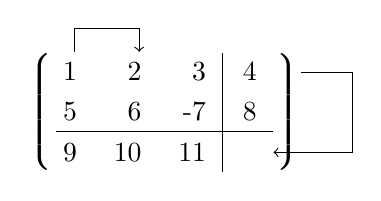
\begin{tikzpicture}[baseline]
        \matrix [
          matrix of math nodes,
          left delimiter={\lgroup},right delimiter={\rgroup},
          nodes in empty cells,
          nodes={inner xsep=0.25em,inner ysep = 0.4em, align=right, anchor=east},
          inner sep=0pt, column sep=.5em,
          %nodes={inner xsep = .2cm, inner ysep = .3cm}
        ] (m) {
         1 & 2 & 3 & 4 \\
         5 & 6 & -7 & 8 \\
         \hline
         9 & 10 & 11 &  \\
        } ;

        \draw (m-1-3.east)+(0,.25) -- (m-3-3.east) -- +(0,-0.25);
      
        \draw[->] (m-1-1.north) -- +(0,.3) -| (m-1-2.north);
        \draw[->] (m-1-4.east)+(1em,0) -- +(1,0) |- (m-3-4.east);
    \end{tikzpicture}
\end{equation*}

\end{document}
